\documentclass{beamer}
\usepackage[utf8]{inputenc}
\usepackage[T1]{fontenc}
% \usepackage{amscd, amsfonts, amsmath, amssymb, amstext, amsthm, caption, epsfig, fancyhdr, float, graphicx, latexsym, mathtools, multicol, multirow, algorithm, chngcntr}
\usepackage[english, french]{babel}
\usepackage{booktabs}

\usepackage{amsmath,amssymb}
\usepackage{graphicx}
\usepackage{caption}
\usepackage{subfig}
\usepackage{xspace}
\usepackage{fourier}


\usepackage{tikz}
\usetikzlibrary{shapes,arrows}
\usepackage{tkz-graph}
\usetikzlibrary{automata,arrows,positioning,calc}
\usetikzlibrary{positioning}
\usetikzlibrary{fit}
\usetikzlibrary{backgrounds}
\usetikzlibrary{calc}
\usetikzlibrary{shapes}
\usetikzlibrary{mindmap}
\usetikzlibrary{decorations.text}
\usetikzlibrary{snakes}

% \theoremstyle{definition} % insert bellow all blocks you want in normal text
% \newtheorem{definition}{Definition}



% tikzmark command, for shading over items
\newcommand{\tikzmark}[1]{\tikz[overlay,remember picture] \node (#1) {};}
% Define block styles
\tikzstyle{decision} = [diamond, draw, fill=blue!20,
    text width=4.5em, text badly centered, node distance=3cm, inner sep=0pt]
\tikzstyle{block} = [rectangle, draw, fill=blue!20,
    text width=5em, text centered, rounded corners]
\tikzstyle{line} = [draw]
\tikzstyle{cloud} = [draw, ellipse,fill=red!20, node distance=3cm,
    minimum height=2em]

\usepackage[most]{tcolorbox}

\setbeamertemplate{blocks}[rounded][shadow=true] % use rounded blocks with standard beamer shadow


% Distributions.
\newcommand*{\UnifDist}{\mathsf{Unif}}
\newcommand*{\ExpDist}{\mathsf{Exp}}
\newcommand*{\DepExpDist}{\mathsf{DepExp}}
\newcommand*{\GammaDist}{\mathsf{Gamma}}
\newcommand*{\LognormalDist}{\mathsf{LogNorm}}
\newcommand*{\WeibullDist}{\mathsf{Weib}}
\newcommand*{\ParetoDist}{\mathsf{Par}}
\newcommand*{\NormalDist}{\mathsf{Norm}}

\newcommand*{\GeometricDist}{\mathsf{Geom}}
\newcommand*{\NegBinomialDist}{\mathsf{NegBin}}
\newcommand*{\PoissonDist}{\mathsf{Poisson}}
\newcommand*{\BivariatePoissonDist}{\mathsf{BPoisson}}
\newcommand*{\CyclicalPoissonDist}{\mathsf{CPoisson}}

\newcommand*{\iid}{\textbf{iid}\@\xspace}
\newcommand*{\pdf}{\textbf{pdf}\@\xspace}
\newcommand*{\cdf}{\textbf{cdf}\@\xspace}
\newcommand*{\pmf}{\textbf{pmf}\@\xspace}
\newcommand*{\abc}{{\textbf{abc}}\@\xspace}
\newcommand*{\smc}{\textbf{smc}\@\xspace}
\newcommand*{\mcmc}{\textbf{mcmc}\@\xspace}
\newcommand*{\ess}{\textbf{ess}\@\xspace}
\newcommand*{\mle}{\textbf{mle}\@\xspace}
\newcommand*{\bic}{\textbf{bic}\@\xspace}
\newcommand*{\kde}{\textbf{kde}\@\xspace}
\newcommand*{\glm}{\textbf{glm}\@\xspace}
\newcommand*{\xol}{\textbf{xol}\@\xspace}
\newcommand*{\cpu}{\textbf{cpu}\@\xspace}
\newcommand*{\gpu}{\textbf{gpu}\@\xspace}
\newcommand*{\arm}{\textbf{arm}\@\xspace}

\def \si {\sigma}
\def \la {\lambda}
\def \al {\alpha}
% \def\e*{\end{eqnarray*}}
\def \di{\displaystyle}

\def \E{\mathbb E}
\def \N{\mathbb N}
\def \Z{\mathbb Z}
\def \NZ{\mathbb{N}_0}
\def \I{\mathbb I}
\def \w{\widehat}
\def \P {\mathbb P}
\def \V{\mathbb V}


\newcommand{\CL}{\mathbb{C}}
\newcommand{\RL}{\mathbb{R}}
\newcommand{\nat}{{\mathbb N}}
\newcommand{\Laplace}{\mathscr{L}}
\newcommand{\e}{\mathrm{e}}
\newcommand{\ve}{\bm{\mathrm{e}}} % vector e

\renewcommand{\L}{\mathcal{L}} % e.g. L^2 loss.

\newcommand{\ih}{\mathrm{i}}
\newcommand{\oh}{{\mathrm{o}}}
\newcommand{\Oh}{{\mathcal{O}}}
\newcommand{\Exp}{\mathbb{E}}

\newcommand{\Norm}{\mathcal{N}}
\newcommand{\LN}{\mathcal{LN}}
\newcommand{\SLN}{\mathcal{SLN}}

\renewcommand{\Pr}{\mathbb{P}}
\newcommand{\Ind}{\mathbb I}
\newcommand\bfsigma{\bm{\sigma}}
\newcommand\bfSigma{\bm{\Sigma}}
\newcommand\bfLambda{\bm{\Lambda}}
\newcommand{\stimes}{{\times}}
\def \limsup{\underset{n\rightarrow+\infty}{\overline{\lim}}}
\def \liminf{\underset{n\rightarrow+\infty}{\underline{\lim}}}




% vertical separator macro
\newcommand{\vsep}{
  \column{0.0\textwidth}
    \begin{tikzpicture}
      \draw[very thick,black!10] (0,0) -- (0,7.3);
    \end{tikzpicture}
}
\newcommand\blfootnote[1]{%
  \begingroup
  \renewcommand\thefootnote{}\footnote{#1}%
  \addtocounter{footnote}{-1}%
  \endgroup
}

% More space between lines in align
% \setlength{\mathindent}{0pt}

% Beamer theme
\usetheme{ZMBZFMK}
\usefonttheme[onlysmall]{structurebold}
\mode<presentation>
\setbeamercovered{transparent=10}

% align spacing
\setlength{\jot}{0pt}

\setbeamertemplate{navigation symbols}{}%remove navigation symbols

\title[BLOCKASTICS I]{Stochastic Models for blockchain analysis}
\subtitle{Blockchain fundamentals and applications}
\author{Pierre-O. Goffard}
\institute[UNISTRA]{UNiversité de Strasbourg\\
 \texttt{goffard@unistra.fr}
}
\date{\today}
% \titlegraphic{\includegraphics[width=2.5cm]{../../../Figures/bfs_logo.png}} 

\begin{document}
\begin{frame}
  \titlepage
\end{frame}
\section{Introduction}
\begin{frame}{Blockchain}
A data ledger made of a sequence of blocks maintained by a achieving consensus in a Peer-To-Peer network.
\begin{columns}
\begin{column}{0.5\textwidth}
% \small

\begin{itemize}
  \item Decentralized
  \item Public/private
  \item Permissionned/permissionless
  \item Immutable
  \item Incentive compatible
\end{itemize}
\end{column}
\begin{column}{0.5\textwidth}
\begin{center}
\begin{tikzpicture}[-, >=stealth', auto, semithick, node distance=01cm]
\tikzstyle{every edge}=[snake=expanding waves,segment length=1mm,segment angle=10, draw]

\tikzstyle{full node}=[circle, fill=tublue,draw=tublue,thick,text=black,scale=0.8]
\tikzstyle{light node}=[circle, fill=white,draw=tublue,thick,text=black,scale=0.8]
\node[full node]    (1)                     {};
\node[full node]    (2)[above right of=1]         {};
\node[full node]    (3)[above left of=1]         {};
\node[full node]    (4)[below of=1]         {};
\node[full node]    (5)[right of=4]         {};
\node[full node]    (6)[below of=4]         {};
\node[light node]    (7)[left of=1]         {};
\node[light node]    (8)[right of=2]         {};
\node[light node]    (9)[left of=4]         {};
\node[light node]    (10)[above right of=5]         {};
\node[light node]    (11)[ right of=5]         {};
\node[light node]    (12)[ below right of=5]         {};
% \node[light node]    (4)[above of=2]         {};
\path

(1) edge node{} (2)
    edge node{} (3)
    edge node{} (7)
    ;
\path
(5) edge node{} (10)
    edge node{} (11)
    edge node{} (12)
    ;
    \path
(4) edge node{} (5)
    edge node{} (1)
    edge node{} (9)
    edge node{} (6)
    ;
    \path
(2) edge node{} (8)   
    ;
\end{tikzpicture}
\end{center}
\end{column}
\end{columns}

\vspace{0.2cm}
We will focus on public blockchain and their associated consensus protocol.
\end{frame}
\begin{frame}{Blocks}
A block contains
\begin{itemize}
  \item block height/ID
  \item Time stamp
  \item hash of the block
  \item hash of the previous block
  \item Set of transactions (data stored in the blockchain)
\end{itemize}
\begin{center}
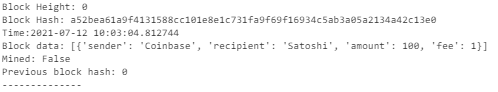
\includegraphics[width=0.9\textwidth]{../../../Figures/genesis_block.png}
\end{center}
\url{https://www.blockchain.com/}
\end{frame}
% \begin{frame}{Cryptographic Hash function}
% \small
% A function that maps data of arbitratry size (message) to a bit array of fixed size (hash value)
% $$
% h:\{0,1\}^\ast\mapsto \{0,1\}^d. 
% $$
% A good hash function is
% \begin{itemize}
% \item deterministic
% \item quick to compute
% \item One way
% \begin{itemize}
%   \scriptsize
% \item[$\hookrightarrow$] For a given hash value $\overline{h}$ it is hard to find a message $m$ such that 
% $$
% h(m) = \overline{h}
% $$
% \end{itemize}
% \item Colision resistant 
% \begin{itemize}
% \item[$\hookrightarrow$] Impossible to find $m_1$ and $m_2$ such that 
% $$
% h(m_1) = h(m_2)
% $$
% \end{itemize}
% \item Chaotic
% $$m_1\approx m_2\Rightarrow  h(m_1) \neq h(m_2)$$
% \end{itemize}

% \end{frame}
\begin{frame}{Consensus protocols}
The mechanism to make all the nodes agree on a common data history.\\
\vspace{0.3cm}
The three dimensions of blockchain systems analysis
\begin{enumerate}
  \item Efficiency (Queueing theory)
  \begin{itemize}
    \item Throughputs
    \item Transaction confirmation time
  \end{itemize}
  \item Decentralization (Entropy)
  \begin{itemize}
    \item Fair distribution of the accounting right
  \end{itemize}
  \item Security (Insurance Risk Theory)
  \begin{itemize}
    \item Resistance to attacks
  \end{itemize}
\end{enumerate}
\footnotesize
\begin{thebibliography}{1}
\bibitem{Fu2020}
X.~Fu, H.~Wang, and P.~Shi, ``A survey of blockchain consensus algorithms:
  mechanism, design and applications,'' {\em Science China Information
  Sciences}, vol.~64, nov 2020.
\end{thebibliography}
\end{frame}
% \begin{frame}{Proof of Work}
% The nodes compete to solve a cryptographic problem by brute force search.
% \begin{tcolorbox}[enhanced,drop shadow, title=PoW]
% \begin{enumerate}
%     \item Draw a random number (nonce)
%     \[
%     X\sim\{1,\ldots, 2^{32}\}.
%     \]
%     \item While $X > L$, where $L$ is the target then try again  
% \end{enumerate}
% \end{tcolorbox}
% \vspace{0.3cm}
% Nodes are chosen according to their computing power
% {\footnotesize
% \begin{thebibliography}{1}
% \bibitem{Na08}
% S.~Nakamoto, ``Bitcoin: A peer-to-peer electronic cash system.'' Available at
%   \href{https://bitcoin.org/bitcoin.pdf}{https://bitcoin.org/bitcoin.pdf},
%   2008.
% \end{thebibliography}  
% }
% \end{frame}
% \begin{frame}{Proof of Stake}
% PoW is slow and ressource consuming. Let $\{1,\ldots, N\}$ be a set of miner and $\{\pi_1,\ldots, \pi_N\}$ be their share of cryptocoins.
% \begin{tcolorbox}[enhanced,drop shadow, title=PoS]
% Node $i\in \{1,\ldots, N\}$ is selected with probability $\pi_i$ to append the next block
% \end{tcolorbox}
% \vspace{0.3cm}
% Nodes are chosen according to what they own.
% \begin{itemize}
%   \item Nothing at stake problem
%   \item Rich gets richer ? (To be discussed later on)
% \end{itemize}
% \footnotesize{
% \begin{thebibliography}{1}

% \bibitem{Saleh2020}
% F.~Saleh, ``Blockchain without waste: Proof-of-stake,'' {\em The Review of
%   Financial Studies}, vol.~34, pp.~1156--1190, jul 2020.

% \end{thebibliography}}

% \end{frame}
\begin{frame}{Applications of blockchain: Cryptocurrency}
\begin{columns}
\begin{column}{0.5\textwidth}
   
{\footnotesize
\begin{thebibliography}{1}
\bibitem{Na08}
S.~Nakamoto, ``Bitcoin: A peer-to-peer electronic cash system.'' Available at
  \href{https://bitcoin.org/bitcoin.pdf}{https://bitcoin.org/bitcoin.pdf},
  2008.
\end{thebibliography}  
}
\end{column}
\begin{column}{0.5\textwidth}  %%<--- here
    \begin{center}
     
\includegraphics[width=0.5\textwidth]{../../../Figures/bitcoin-6284869_1920.png}
     \end{center}
\end{column}
\end{columns}

\begin{itemize}
  \item Transaction anonymity
  \item No need for a thrusted third party
\end{itemize}
\end{frame}

\begin{frame}{How does it work?}
\begin{enumerate}
  \item No central authority (Decentralized network)
  \item Ledger to record all the transactions and coin ownership (blockchain)
  \item A coin generation process (block finding reward)
    \begin{itemize}
    \item[$\hookrightarrow$] Incentive to the full nodes 
  \end{itemize}
  \item Ownership can be proved cryptographically (wallet associated to a public/private key)
  \item Transactions can be issued by an entity proving ownership of the cryptographic unit (through the private key) 
  \item The system cannot process more than one transaction associated to the same cryptographic unit (double spending)
\end{enumerate}
\tiny
\begin{thebibliography}{1}

\bibitem{Lansky2018}
J.~Lansky, ``Possible state approaches to cryptocurrencies,'' {\em Journal of
  Systems Integration}, vol.~9, pp.~19--31, jan 2018.

\end{thebibliography}
\end{frame}
\section{Consensus protocols}
\begin{frame}{Consensus protocol}
\begin{tcolorbox}[enhanced,drop shadow, title=Definition]
    Algorithm to allows the full nodes to agree on a common data history
\end{tcolorbox}
It must rely on the scarce resources of the network
\begin{itemize}
  \item bandwidth
  \item computational power
  \item storage (disk space)
\end{itemize}
\end{frame}
\begin{frame}{Types of consensus protocols}
\begin{enumerate}
  \item Voting based 
  \footnotesize
\begin{thebibliography}{1}

\bibitem{lamport1982the}
L.~Lamport, R.~Shostak, and M.~Pease, ``The byzantine generals problem,'' {\em
  ACM Transactions on Programming Languages and Systems}, pp.~382--401, July
  1982.

\end{thebibliography}
\normalsize
  \item Leader based
  \begin{itemize}
    \item Proof-of-Work (computational power)
    \item Proof-of-Stake (tokens)
  \end{itemize}
\end{enumerate}
\end{frame}


\section{Decentralized Finance (and insurance)}



\end{document}
